\fancyhead[LO, RE] {Analisi e Pianificazione}
\section{Analisi e Pianificazione}
\subsection{Analisi del contesto}
I motivi principali per cui si stesse discutendo un approccio diverso al trasferimento dei dati relativi al progetto CRM, erano legati alla eccessiva dispersività del progetto esistente, che crea molti file di testo e necessita dell'affidamento ad un fornitore che si occupi del caricamento dei dati nei database relativi ad ogni stato (Italia, USA e Giappone).\\
La natura del sistema esistente era tale da consistere di schedulazioni impostate a diverse fasce orarie da parte di aziende diverse. La prima schedulazione era relativa alla creazione dei file da parte di Industries, e la seconda era impostata dal fornitore a 6 ore di distanza, di comune accordo, per il caricamento effettivo dei dati. Sebbene l'esecuzione del programma di Industries che genera i file fosse molto breve, si era deciso di mantenere un discreto margine di tempo per intervenire in caso di errori prima del caricamento dei dati da parte del fornitore.\\
Nell'ottica di interrompere le relazioni con tale fornitore, si è deciso di considerare l'ipotesi di caricare i dati direttamente nei database a cui si riferiscono gli showroom, avendone nel tempo ottenuto l'accesso diretto. Tali database sono di proprietà di un fornitore che si occupa della creazione anche dei software installati nei vari punti vendita, principalmente tablet, grazie ai quali i vari clienti possono visualizzare il campionario ed eseguire gli evenutali ordini. Gli ordini dei clienti vengono poi trasferiti nello stesso modo dei caricamenti, sempre via file e tramite un fornitore, con un processo inverso rispetto a quello della popolazione dei database con i campionari, generando dei report interni ad Industries, tramite Oracle Reports di cui l'azienda possiede la licenza.

\subsection{Piano di Lavoro}
 Piano di lavoro

Lo stage svolto in azienda ha avuto una durata stabilita di circa 310 ore, suddivise in 10 settimane da 4 giorni, alla fine della maggior parte delle quali era prevista una milestone.
\newpage
\subsubsection{Pianificazione delle attività}
La pianificazione delle attività è stata la seguente:
\begin{longtable}{| c | c |}%{| p{.20\textwidth} | p{.80\textwidth} |}
	
	\hline
	\textbf{Settimana} & \textbf{Task} \\ \hline

	06-09 Agosto (1a Settimana) &  \begin{tabular}{@{}c@{}@{}@{}@{}@{}}  Studio del programma esistente \\relativo all'export delle informazioni \\necessarie al CRM,  con supporto \\  degli sviluppatori di quel  \\  progetto (16h) e creazione di\\ schemi riassuntivi (16h). \end{tabular}\\ \hline      

	21-23 Agosto (2a Settimana) &  \begin{tabular}{@{}c@{}@{}@{}@{}} Studio del programma esistente \\relativo alla fase di import ordini,\\ con supporto degli sviluppatori  \\di quel progetto (16h) e \\ creazione schemi riassuntivi (16h).\end{tabular}\\ \hline          

	27-30 Agosto (3a Settimana)  &  \begin{tabular}{@{}c@{}@{}@{}@{}}  Analisi ed eventuali test delle diverse \\modalità offerte dal mercato per il \\passaggio dei dati (28h) e discussione \\con il Responsabile riguardo\\ la validità della scelta(4h).\end{tabular}\\ \hline

	03-06 Settembre (4a Settimana)  &  \begin{tabular}{@{}c@{}@{}@{}}  Sviluppo di una versione dimostrativa\\   del programma di export con la nuova\\ tecnologia, con funzionalità e set\\ di dati minime (32h). \end{tabular}\\ \hline

	10-13 Settembre (5a Settimana) &  \begin{tabular}{@{}c@{}@{}@{}}  Sviluppo di una versione dimostrativa\\   del programma di export con la nuova\\ tecnologia, con funzionalità e set\\ di dati minime (32h). \end{tabular}\\ \hline


	17-20 Settembre (6a Settimana) & \begin{tabular}{@{}c@{}@{}}   Stesura documentazione tecnica di \\rilascio della versione dimostrativa\\ di export (32h). \end{tabular}\\ \hline
  

	24-27 Settembre (7a Settimana) &\begin{tabular}{@{}c@{}@{}}   Sviluppo di una versione dimostrativa\\ del programma di export con la nuova\\ tecnologia, con funzionalità e set\\ di dati minime (32h) \end{tabular}\\  \hline

	01-04 Ottobre (8a Settimana) & \begin{tabular}{@{}c@{}@{}}   Sviluppo di una versione dimostrativa\\ del programma di export con la nuova\\ tecnologia, con funzionalità e set\\ di dati minime (32h) \end{tabular}\\  \hline

	08-11 Ottobre (9a Settimana) & \begin{tabular}{@{}c@{}@{}}   Stesura documentazione tecnica di \\rilascio della versione dimostrativa\\ di import (32h). \end{tabular}\\ \hline

	15-18 Ottobre (10a Settimana) & \begin{tabular}{@{}c@{}@{}@{}@{}@{}@{}} Verifica ed unione delle documentazioni \\(16h) e discussione con il Responsabile ed i \\Service Manager sulla qualità del prodotto\\sviluppato, fattibilità in termini di\\ tempistiche e complessità, e sul'eventuale \\realizzazione del  progetto per\\ la prossima campagna vendite (4h)\end{tabular}\\ \hline      

	\caption{Pianificazione: Distribuzione Settimanale}

\end{longtable}

\begin{figure}[!h]
\thispagestyle{empty}
\centering
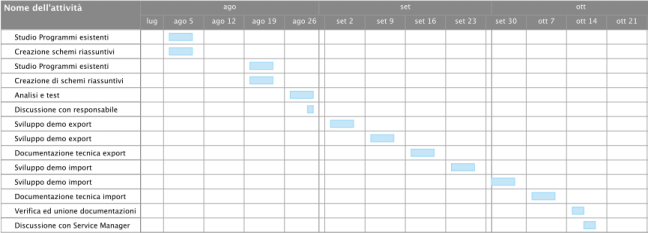
\includegraphics[scale=0.85]{img/Gantt.png}
\caption{Diagramma delle attività}
\end{figure}
\newpage

\subsubsection{Obiettivi}
Gli obiettivi dello stage sono codificati con le seguenti notazioni:
\begin{itemize}
\item <min> per gli obiettivi minimi, vincolanti in quanto richieste primarie del committente;
\item <max> per gli obiettivi massimi, inclusi quelli desiderabili ed opzionali, non vincolanti o strettamente necessari, ma dal riconoscibile valore aggiunto;
\item <for> per gli obiettivi formativi, rappresentanti valore aggiunto in termini culturali e di conoscenze da acquisire dallo stagista.
\end{itemize}

\chapter{Minimi}
\begin{itemize}
\item Min1: Reverse Engeneering del software di interfaccia attuale;
\item Min2: Individuazione della corretta architettura necessaria per la nuova implementazione;
\item Min3: Autonomia nei test di estrazione ed importazione dati su Sql Server.
\end{itemize}

\chapter{Massimi}
\begin{itemize}
\item Max1: Capacità di ottimizzazione dei processi;
\item Max2: Superamento dei bugs e dei limiti contenuti nei programmi esistenti;
\item Max3: Individuazione delle soluzioni alle problematiche rilevate.
\end{itemize}

\chapter{Formativi}
\begin{itemize}
\item Acquisizione di abilità funzionali sulla gestione degli orgini su ERP;
\item Acquisizione di conoscenze tecniche su strumenti di ETL;
\item Interazione con i Service Manager;
\item Stesura di documentazione Tecnica.
\end{itemize}